\section{РАЗРАБОТКА ПРОГРАММНЫХ МОДУЛЕЙ}
\label{sec:dev}

Основная практическая состовляющая данной работы состоит в непосредственной разработки системы для редактирования трехмерных моделей. Ниже приведены различные ключевые элементы
разработки данной системы, методология, использованная при разработке кода отображения трехмерной графики -- шейдеров для материалов, разработка методов автоматизации сборки
системы а также подходы, использованные при разработке пользовательского интерфейса системы.

\subsection{Разработка шейдеров и кода отображения аппаратной графики}
\label{sub:dev:shader}
Шейдер (англ. shader — затеняющая программа) — компьютерная программа, предназначенная для исполнения процессорами видеокарты (GPU).
Шейдеры составляются на одном из специализированных языков программирования и компилируются в инструкции для GPU.

\subsection{Методология использования компоновщика Webpack}
\label{sub:dev:webpack}
Для сборки проекта в пакет, пригодный для использования на пользовательском компьютере был выбран компоновщик Webpack\cite{webpack}\cite{webpack2}, помогающий тривиализировать сложную задачу
автоматизации построения релизного пакета приложения. Функционал Webpack упрощает процесс разработки одностраничных приложений, реализуя функционал продвинутого
разделения кода и <<горячей перезагрузки ресурсов>> (Hot Reload) для более быстрой разработки с помощью компонентной технологии пользовательского интерфейса, такой как React.
Webpack -- система сборки, которая предоставляет не только функционал компоновки модулей, но и может выполнять задачи, которые обычно выполняют специализированные task-runner системы,
такие как Gulp или Grunt. К тому же, возможности Webpack не ограничиваются обработкой JavaScript-файлов, так как он может работать с любыми видами статических ресурсов веб среды:
CSS (и языки, транслируемые в CSS), изображения, html-компоненты и, после реализации соответствующего модуля-загрузчика, любой другой тип содержимого. Webpack также поддерживает
полезную при разработки сложных веб-приложений функцию -- code splitting (разбиение кода) и dependency tree shaking (прочесывания дерева зависимостей). Большое приложение можно
разбить на подмодули и система упаковки автоматически включит их в скомпилированный ресурсный файл, в случае если он используется где-либо в системе. Все ненужные ресурсы не попадают
в результирующий исполняемый файл кроме случаев, когда это явно указано в конфигурации webpack (например, в случаях зависимости времени выполнения без соответствующей зависимости на
этапе компиляции).

Компоновщик Webpack позволяет упаковывать, компилировать, организовывать множество ресурсов и библиотек, необходимых для современного веб-проекта. Схема сборки веб проекта посредством
модулей-загруз-чиков представлена на рисунке \ref{figure:domain:webpack}.

\begin{figure}[ht]
\centering
  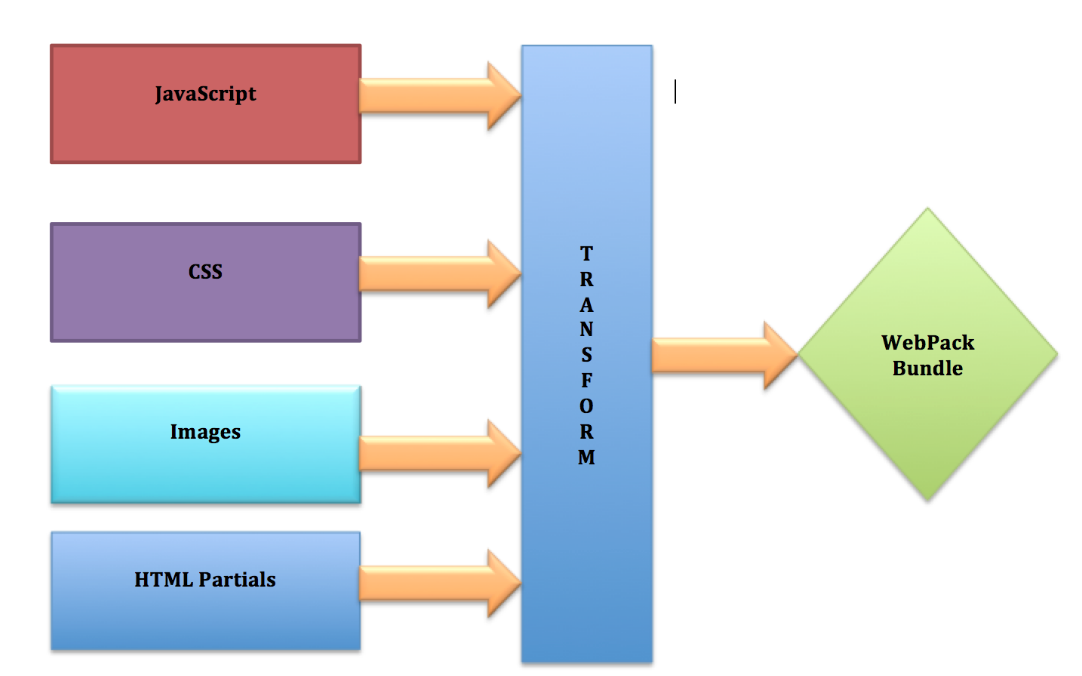
\includegraphics[scale=0.40]{webpack.png}
  \caption{Схема процесса сборки webpack}
  \label{figure:domain:webpack}
\end{figure}

Стандартные возможности Webpack включают, но не ограничиваются следующими:
\begin{itemize}
\item автоматическое построение дерева зависимостей ресурсов, в том числе зависимостей разных типов содержимого друг от друга (например, зависимости *.jsx или *.mjs файлов от каскадных таблиц
стилей *css или их прародителей, *.less/*.sass);
\item упаковка модулей, поддерживающих возможности ленивой (deferred, lazy loading) загрузки в отдельные файлы;
\item выполнение оптимизации кода, удаление ненужных элементов дерева зависимостей и минимизация получившихся исполняемых файлов;
\item поддержка функционала локального сервера ресурсов (dev server), позволяющего производить <<горячую перезагрузку ресурсов>> на странице прямо в процессе работы над проектом, что достигается
путем частичной перекомпиляции некоторых из ветвей зависимостей проекта.
\end{itemize}

Пример использования средств Webpack для организации автоматизированной сборки проекта:

Как и большинству инструментов Web-разработки, Webpack реализован на базе API Node.js \cite{wamp}\cite{node} -- серверной реализации JavaScript, построенной на базе движка V8. Установка Webpack производится с помощью
системы управления модулями node.js -- NPM \cite{npm} (Node package manager). Установка производится с помощью следующей команды в терминале:

\begin{lstlisting}[language=bash, label=lst:domain:html]
npm install webpack --global
\end{lstlisting}

Данная команда установит Webpack глобально в системе (по умолчанию установив его в директорию /usr/local/bin/npm/node\_modules), создав символические ссылки на необходимые исполняемые файлы, что
позволит запускать его из любой директории на компьютере разработчика. Далее, внутри директории проекта, был создан файл index.html с начальной разметкой:

\begin{lstlisting}[language=HTML, label=lst:domain:html]
<html lang="ru">
<head>
  <meta charset="UTF-8">
</head>
<body>
  <h2></h2>
  <script src="bundle.js"></script>
</body>
</html>
\end{lstlisting}

Важной частью этого кода является ссылка на файл bundle.js, который содержит в себе результат работы Webpack.
Первый файл определяет начальную точку приложения, в которой Webpack будет искать все зависимости. Это сработает и в том случае, если в вызываемых зависимостях 
есть свои зависимости от других модулей -- до тех пор, пока не подключатся абсолютно все необходимые модули. Таким образом, на выход получится один файл bundle.js со всем модулями.
В проекте была собрана конфигурация webpack с React.js

Точка входа в приложение:
\begin{lstlisting}[language=TypeScript, label=lst:domain:html]
const config = {
  entry: {
    app: './src/js/app.js'
  }
\end{lstlisting}

Параметры финальной упаковки:
\begin{lstlisting}[language=TypeScript, label=lst:domain:html]
  output: {
    filename: 'bundle.js',
    path: distPath
  }
\end{lstlisting}

Одной из самых важных особенностей Webpack, является возможность использовать loader. Loader по сути своей являются аналогами “задач” (tasks) в Grunt и Gulp. По существу,
они принимают содержимое файлов, а затем преобразуют его необходимым образом и включают результат преобразования в общую сборку.
Подключение React.js в бандлере:
\begin{lstlisting}[language=TypeScript, label=lst:domain:html]
 module: {
    rules: [{
      test: /\.js$/,
      exclude: [/node_modules/],
      use: [{
        loader: 'babel-loader',
        options: {
          presets: ['env', 'react']
        }
      }]
    }.
\end{lstlisting}

Для увелечения гибкости стиля был выбран язык SASS\cite{sass}\cite{sass2}\cite{sass3}. SASS это язык похожий на HAML (весьма лаконичный шаблонизатор), но предназначенный 
для упрощения создания CSS-кода. Проще говоря, SASS это такой язык, код которого специальной ruby-программой транслируется в обычный CSS код. Синтаксис этого языка очень гибок, 
он учитывает множество мелочей, которые так желанны в CSS. 
Изменение файла конфигурации для подключение подгрузки стилей:

\begin{lstlisting}[language=TypeScript, label=lst:domain:html]
test: /\.scss$/,
      exclude: [/node_modules/],
      use: extractSass.extract({
        fallback: 'style-loader',
        use: [{
          loader: 'css-loader',
          options: {
            modules: true,
            sourceMap: true,
            importLoaders: 2,
            localIdentName: '[name]__[local]__[hash:base64:5]', // className template
            minimize: isProduction
          }
        },
          'sass-loader',
          'resolve-url-loader'
        ]
      })
\end{lstlisting}

Для работы с изображениями мы будем использовать url-loader, который является ещё одним loader для Webpack. Он берёт относительные URL 
ваших изображений и изменяет их таким образом, чтобы они корректно подключались в общем файле.
\begin{lstlisting}[language=TypeScript, label=lst:domain:html]
test: /\.(gif|png|jpe?g|svg)$/i,
      use: [{
        loader: 'file-loader',
        options: {
          name: 'images/[name][hash].[ext]'
        }
      }, {
        loader: 'image-webpack-loader',
        options: {
          mozjpeg: {
            progressive: true,
            quality: 70
          }
        }
      },
      ],}, {
      test: /\.(eot|svg|ttf|woff|woff2)$/,
      use: {
        loader: 'file-loader',
        options: {
          name: 'fonts/[name][hash].[ext]'
        }
      },
    }]
  }
\end{lstlisting}


\subsection{Подходы к разработке пользовательского интерфейса}
\label{sub:dev:react}
React (иногда React.js или ReactJS)\cite{react} — JavaScript-фреймворк с открытым исходным кодом для разработки пользовательских интерфейсов.
React разрабатывается и поддерживается Facebook, Instagram и сообществом отдельных разработчиков и корпораций.React может использоваться для 
азработки одностраничных и мобильных приложений. Его цель — предоставить высокую скорость, простоту и масштабируемость. В качестве библиотеки для разработки 
пользовательских интерфейсов, React часто используется с другими библиотеками, такими как Redux.
Сравнивать ReactJs с Angular или другими MVC фреймворками не имеет смысла, так как ReactJs – это только представление. React – это язык шаблонов в сочетании 
несколькими функциями, которые позволяют отрисовать HTML, т.е. результат работы React – это HTML. ReactJs реализует концепции реактивного программирования: изменение 
результата работы зависит от состояния компонентов. Так, A = B + C, и результат A всегда будет зависеть от значений B и C. ReactJs постоянно работает с DOM, перерисовывая 
его при изменении условий (та часть DOM, которую меняет ReactJs, называется компонентом). 
React разработан вокруг концепции многоразовых компонентов. Вы определяете небольшие компоненты, и объединяете их, чтобы сформировать более крупные компоненты.
Все компоненты, маленькие или большие, могут использоваться повторно, даже в разных проектах.

\subsubsection{Обоснование выбора библиотеки React}
Поскольку пользовательский интерфейс пользователя является полностью компонентной структурой\cite{genesisgui}, для ее реализации более естественно подходят компонентные фреймворки, позволяющие
реализовать дерево зависимостей, направленное сверху вниз (от больших уровней абстрации к более низким). Такая архитектура системы пользовательского интерфейса позволяет добиться лучшей расширяемости
и избежать гонок за право манипулации состоянием системы ввиду использования подхода <<Единого источника истины>> (Single source of truth). Компонентный пользовательский интерфейс также реализуется
в таких фреймворках, как vue.js и angular, однако в качестве основного был выбран React ввиду его первичности на рынке средств разработки GUI и развитого набора средств работы с парадигмой Redux.

\subsubsection{Создание компонента Button}

\begin{lstlisting}[language=TypeScript, label=lst:domain:typescript]
function Button (props) {

 return <button type="submit">{props.label}</button>;

}

ReactDOM.render(<Button label="Save" />, mountNode)
\end{lstlisting}

Важной особенностью ReactJs\cite{react2}\cite{react3} является использование JSX. Это надстройка на JS, позволяющая использовать про-XML синтаксис в 
Javascript коде. JSX – это сочетание javascript и html, которые в связке являются непривычным синтаксисом для большинства разработчиков. 
Стандартом считается разделение JS части от разметки, что усложняет слежение за изменениями HTML -> JS -> HTML. JSX позволяет видеть все процессы 
в одном месте, не отвлекаясь на сложности грамотного и валидного кода. После компиляции JSX получается чистый JS.

\begin{lstlisting}[language=TypeScript, label=lst:domain:typescript]
const InputForm = React.createElement(
 "form",
 { target: "_blank", action: "https://google.com/search" },
 React.createElement("div", null, "Enter input and click Search"),
 React.createElement("input", { className: "big-input" }),
 React.createElement(Button, { label: "Search" })
);
function Button (props) {
 return React.createElement(
   "button",
   { type: "submit" },
   props.label
 );
}
ReactDOM.render(InputForm, mountNode);
\end{lstlisting}

JSX запись соответсвующего компонента по своему внешнему виду напоминает HTML, встроенный в JavaScript, однако существует ряд ограничений на их определение.
Например, RSX ReactDOM компоненты не могут быть определены как список XML элементов -- обязательно наличие корневого XML элемента, оборачивающего все дочерние элементы.
В случае, когда необходимо вернуть из функции или передать в рендер-функцию набор элементов, они передаются в виде JavaScript Array, где у каждого элемента обязательно должно
быть установлено свойство <<key>>, необходимое для инкрементальной реиндексации дерева элементов. Свойство key должно быть уникально в рамках коллекции, поэтому его, как правило,
привязывают к случайному guid элементу, либо к хэш сумме неизменяемых элементов отображаемого компонента. Такой подход позволят эффективно перерисовывать дерево элементов
и отслеживать появление в дереве компонентов новых листьев.

\begin{lstlisting}[language=TypeScript, label=lst:domain:typescript]
const InputForm =
 <form target="_blank" action="https://google.com/search">
   <div>Enter input and click Search</div>
   <input className="big-input" name="q" />
   <Button label="Search" />
 </form>;

function Button (props) {
 return <button type="submit">{props.label}</button>;
}
ReactDOM.render(InputForm, mountNode);

\end{lstlisting}

\subsubsection{Преимущества использования React}

Использование изоморфного подхода помогает производить рендеринг страниц быстрее, тем самым позволяя пользователям чувствовать 
себя более комфортно во время работы с приложением. Поисковые системы индексируют такие страницы лучше. Поскольку один и тот же код может 
быть использован как в клиентской, так и в серверной части приложения, нет необходимости в дублировании одного и того же функционала. В результате время 
разработки и затраты снижаются
Virtual DOM может повысить производительность высоконагруженных приложений, что может снизить вероятность возникновения возможных неудобств и улучшает 
пользовательский опыт. Благодаря переиспользованию кода стало гораздо проще создавать мобильные приложения. Код, который был написан во время создания сайта, 
может быть снова использован для создания мобильного приложения. 

\subsubsection{Изоморфные приложения}

Изоморфные приложения или изоморфный JavaScript, это использование одно и того же кода как в серверной, так и в клиентской части приложения. При открытии 
сайта в браузере, содержимое страницы должно быть загружено с сервера. В случае с SPA-приложениями (Single Page Application), это занимает некоторое время. Во время загрузки 
пользователи видят либо пустую страницу, либо анимацию загрузки. 

\begin{figure}[ht]
\centering
  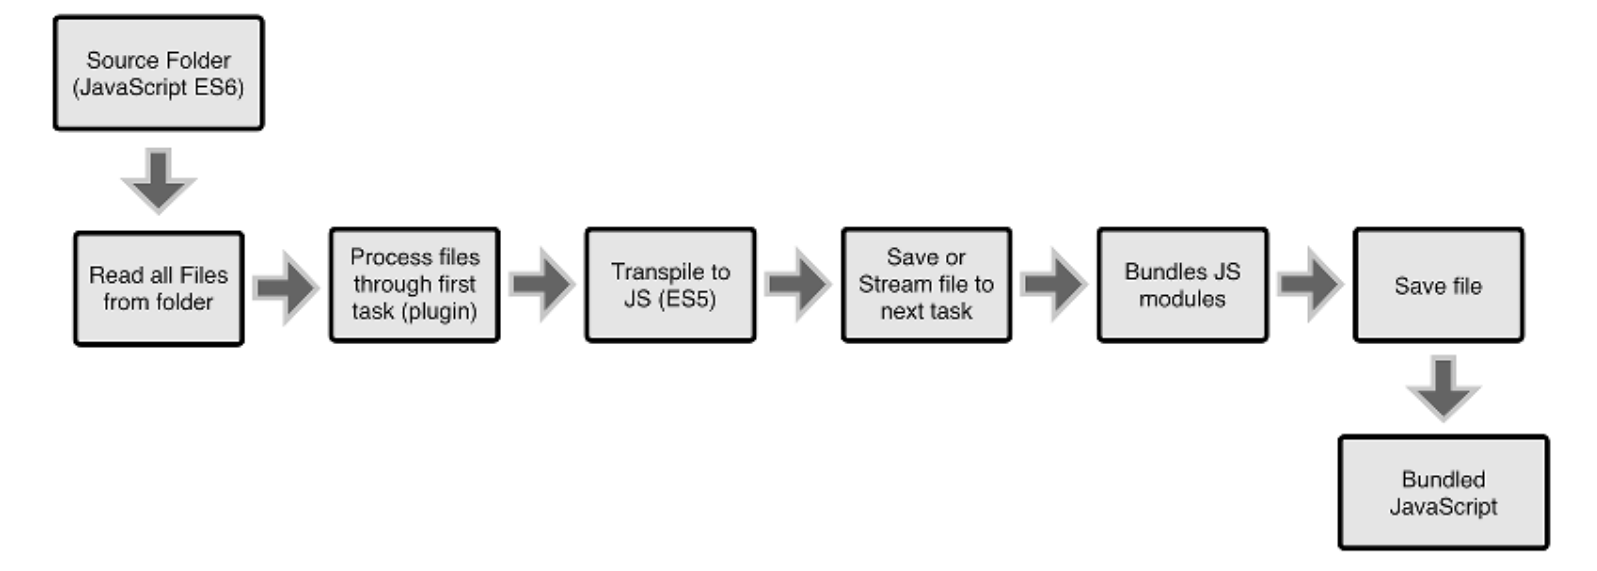
\includegraphics[scale=0.30]{react.png}
  \caption{Процесс загрузки изоморфных приложений}
  \label{figure:domain:react}
\end{figure}

Учитывая, что по современным стандартам ожидание в течение более чем двух секунд может быть весьма заметным неудобством для пользователя, сокращение времени загрузки 
является крайне важным преимуществом. Еще одна весомая проблема: поисковые машины плохо индексируют SPA-приложения. Исполнение JavaScript кода на стороне сервера исправляет 
подобную проблему. В случае с изоморфным приложением после загрузки страницы будет продолжаться рендеринг компонентов. Такая возможность рендеринга страниц как на сервере, так и 
на клиенте приводит к заметным преимуществам, таким как возможность лучшего индексирования страниц поисковыми машинами и улучшение пользовательского опыта. Более того, такой подход 
позволяет снизить время, затрачиваемое на разработку. При использовании некоторых современных фреймворков, вы должны создавать компоненты, которые должны рендериться на стороне сервера, 
а также шаблоны для клиентской стороны приложения. С помощью React можно создавать компоненты, которые работают на обеих сторонах.

\subsubsection{Document Object Model}

Document Object Model, или DOM, — это способ представления и взаимодействия с объектами в HTML, XHTML и XML документах. Согласно этой модели, каждый такой документ
представляет собой иерархическое дерево элементов, называемое DOM-деревом. Используя специальные методы, можно получить доступ к определенным элементам документа и 
изменять их в зависимости от нужных требований. При создании динамичной интерактивной веб-страницы необходимо, чтобы DOM обновлялся так быстро, как это возможно после 
изменения состояния определенного элемента. Для данной задачи некоторые фреймворки используют прием, который называется «dirty checking» и заключается в регулярном опросе 
состояния документа и проверке изменений в структуре данных. Подобная задача может стать самой настоящей проблемой в случае высоконагруженных приложений. Virtual DOM, в свою 
очередь, хранится в памяти. Именно поэтому в момент, когда «настоящий» DOM меняется, React может изменять Virtual DOM в мгновение ока. React «собирает» такие изменения сравнивает 
их с состоянием DOM, а затем перерисовывает изменившиеся компоненты.

При данном подходе не производится регулярное обновление DOM. Именно поэтому может быть достигнута более высокая производительность React приложений. Второе следствие вытекает 
из изоморфной природы React: можно производить рендеринг на стороне сервера совсем как на стороне клиента.

Для создания UI-интерфейса создается структура файлов и папок

\begin{lstlisting}[language=bash, label=lst:domain:typescript]
+-- js 
|   +-- react 
|       +-- react-dom.js 
|       +-- react.js 
|   +-- app.js 
+-- index.html 
+-- package.json 
+-- server.js
\end{lstlisting}

Babel\cite{babel} — это компилятор, который транслирует любой диалект JavaSc-ript, включая CoffeeScript, TypeScript и другие надстройки над языком в 
JavaScript ES5, который поддерживается почти всеми браузерами, включая IE8, если добавить babel-polyfill. Сила Babel в его модульности и расширяемости 
за счет плагинов. Например, уже сейчас можно использовать самые последние изменения JavaScript, не переживая, что они не будут работать в старых браузерах.
Для трансляции компонентов React в проекте можно использовать пресет babel-preset-react. Чтобы наш код корректно работал в старых браузерах, необходима установка 
пакета babel-polyfill, а babel-preset-es2015 и babel-preset-stage-0 необходимы, чтобы писать на ES6/ES7 диалектах соответственно.

\begin{lstlisting}[language=bash, label=lst:domain:typescript]
npm i --save babel-core
    babel-plugin-transform-decorators-legacy
    babel-polyfill 

babel-preset-es2015
    babel-preset-react babel-preset-stage-0
\end{lstlisting}

Эти зависимости надо устанавливать как зависимости проекта, так как серверной части приложения тоже нужен babel.
При запуске babel будет обращаться к файлу .babelrc в корне проекта, в котором хранится конфигурация и список используемых preset'ов и плагинов.

\begin{lstlisting}[language=TypeScript, label=lst:domain:typescript]
{
  "presets": [
    "es2015",
    "react",
    "stage-0"
  ],
  "plugins": [
    "transform-decorators-legacy"
  ]
}
\end{lstlisting}

\subsubsection{Локальный сервер} 

С помощью Node.js* и express был создан локальный сервер. 

\begin{lstlisting}[language=TypeScript, label=lst:domain:typescript]
require('babel-core/register');
['.css', '.less', '.sass', '.ttf', '.woff', '.woff2'].forEach((ext) => require.extensions[ext] = () => {});
require('babel-polyfill');
require('server.js'); 

var express = require('express'); 
var app = express(); 
app.set('port', (process.env.PORT || 3000)); 
app.use('/', express.static(__dirname)); 
app.listen(app.get('port'), function() { console.log('Server started: http://localhost:' + app.get('port') + '/'); });
\end{lstlisting}

В файле package.json в секция scripts, прописываем команду start. 
Cервер запускаем с помощью команды npm start, 
Такой вариант использовать удобнее чем, когда для запуска сервера, вам приходится писать гораздо больше, например:
node server.js -option1 -option2 CONST=qweqwe ... 

\subsubsection{React и ReactDOM}

ReactDOM -- одна из инновативных особенностей фреймворка React, обеспечивающая высокую производительность при работе с графическим интерфейсом пользователя.
По своей сути является представлением дерева компонентов системы в памяти, позволяя достичь минимального обновления фактического DOM за счет вычисления состояний компонентов в памяти.
ReactDOM поддеживает изменение устройства компонентов посредством манипуляций над двумя из его внутренних хранилищ состояния: свойствами (props), и переменным состоянием (state). ReactDOM
обеспечивает эффективную переорганизацию структуры компонентов в результате изменения перечисленных хранилищ посредством пересчета вида только изменившихся ветвей дерева.

Для того чтобы произвести установку соответствующих библиотеки используются следующие вызовы в терминале bash либо powershell:

\begin{lstlisting}[language=bash, label=lst:domain:typescript]
npm i --save react react-dom
\end{lstlisting}

Также требуется установка react-hot-loader: при изменении исходного кода компонентов в процессе разработки, браузер будет перезагружать страницу автоматически. 

\begin{lstlisting}[language=bash, label=lst:domain:typescript]
npm i --save-dev react-hot-loader
\end{lstlisting}

Начиная с 3 версии, react-hot-loader рекомендовано прописывать в .babelrc в качестве одного из плагинов. Ранее же он передавался в конфигурацию webpack 
в качестве одного из конвейеров для JavaScript-файлов.

\begin{lstlisting}[language=bash, label=lst:domain:typescript]
---   "transform-decorators-legacy"
+++ "transform-decorators-legacy",
+++ "react-hot-loader/babel"
\end{lstlisting}
